INTRO

%In the introduction: Summarize the findings Make a paragraph about why Mexico is an interesting case. It would be nice if here, and also throughout the chapter, you could try to link results/the case to separation-of-power overall. Does Mexico fall closer to the American-type or to the Brazilian multiparty type? How does this impact debate? In the introduction, you need to polish the language- English is high quality but it reads a bit too informal at times in the intro.

Why Mx interesting
(1) Single-term limits lifted
(2) Presidential system with three parties
(3) div/unif gov
(4) 


Legislative studies are a relatively young field of Mexican politics. Its growth is remarkable, with new research on candidate selection \citep{ascencio.kerevel.cand-sel-beh.2021}; elections and redistricting \citep{magar.altman.mcd.trelles2016pg}; the standing committee system \citep{bejar.Comisiones2009ed.book}; party discipline \citep{tellez-del-rio.2018}; vote trading \citep{lopez.lara.aldf2013}; pork barreling \citep{kerevelPork2015}; procedure and instability \citep{heller.weldon.2003}; gubernatorial influences in roll call voting \citep{rosas.langston.2011}; constitutional amendment \citep{casar.marvan2014book}; executive success \citep{bejarQuienLegisla2012} and conditions for predominance \citep{weldon.1997}; agenda setting \citep{casar.agsetting.2016}; the budget process \citep{weldon.2002}, and more.

But there is no scholarship on legislative debate in sight. Other than brief and general mentions to the subject, I could find no systematic study of floor access. This chapter takes a step towards filling in this gap by describing the institutions of speech in the Cámara de Diputados and performing a systematic examination of the determinants of floor participation.

The case should raise interest beyond area specialists. Mexico has a separation of powers constitution that has experienced divided and unified government in recent years. The three-and-a-half party system is distinct from both North American dualism and systems with extreme fragmentation, such as Brazil. And Mexico recently dropped single-term limits for members of Congress. \citet{proksch-slapin2015book} theorize that personal vote incentives make legislators organize the assembly with high levels of autonomy in floor debate. With little intra-party competition, such incentives were mostly absent in Mexico, but are bound to increase due to electoral reform. 

The chapter uncovers a tension between formal and informal speech institutions. Formal rules decentralize agenda power by granting members broad rights of recognition to take the floor and deliver speeches. Informal rules channel debate through legislative parties, leaders managing participation in a centralized fashion. The empirical analysis reveals systematic effects of predictors associated with party hierarchies (such as leaders, committee chairs, and majority status) and predictors tied to individual candidate promotion (such as incumbents elected in single-member districts and the prospect of reelection) in the number and length of the speeches that members of Congress deliver. 

Focus is on the Cámara de Diputados of the bicameral Congress. The chambers have symmetric powers over most legislation, but the Senate is excluded from adoption of the annual budget, and I leave it out. Moreover, due to time constraints, I further narrow the focus to three out of eight Cámara terms since the advent of competitive politics in Mexico. I examine the 60th Legislature (2006-09), the 62nd (2012-15), and the 64th (2018-21) up to the end of the second ordinary year---enough to investigate how the recent removal of term limits affects debate.

The chapter is organized thus. Section 2 describes political institutions, the party system, and major changes to both. Section 3 describes the institutional setting of debate in the Cámara. It identifies key players, the structure of debate, recognition-granting motions, and how party discipline works as a substitute to centralized agenda power. Section 4 performs data analysis. Multiple regression models are fit on the universe of speech in the three periods observed. Section 5 discusses Mexican speech institutions in comparison to stylized versions of the U.K. Parliament and the U.S. Congress. Section 6 concludes. 





CONC

Tension lies at the heart of legislative debate in the Cámara. On one hand, parties have informally, but effectively managed to reign in members' capacity to take the floor. The effects that the chapter's regression models uncovered for the majority, for leaders, and for committee chairs are all channeled through party structures in the Junta. On the other hand, formal rules grant individual members rights of recognition to take the floor and, we have seen, these take many guises. The effect attributable to SMDs after the removal of term limits is, in all likelihood, associated to renovated personal vote incentives that members face. 

Whether or not the informal solution to avoid plenary bottlenecks will continue to operate as it has so far in the Cámara is uncertain. Little intra-party competition used to remove personal vote incentives that leads members to differentiate by taking the floor in Proksch and Slapin's model. With the removal of term limits, incumbents with static ambition may soon start overwhelming the system by exploiting the formal autonomy of floor debate in their need to strengthen their electoral connection.

It is important to keep in mind that the place of debate in the legislative process /follows/ negative agenda filters. Agenda-setting mechanisms let leaders prevent consideration of motions when they anticipate debate to go in undesired directions---speakers opening issues that threaten to divide the majority. If parties can no longer prevent plenary bottlenecks, pressure to reform the rules will inevitably build up. Reform could give leaders formal ex-ante vetoes to prevent consideration (and debate) of unwanted legislation, by removing the formal rights that render floor access permeable, or both. 

%But secondary is not the same as unimportant. Position taking is a central activity in electoral connection \citep{mayhew.1974} and home style \citep{fenno.1978} models of political ambition. And plenary debate is the chief position taking tool in the chamber. 

%The collapse of the three-party system in 2018 also plays against. Perhaps the heterogeneous coalition that gave Morena unified control of government will manage to consolidate, imposing a new informal arrangement, in spite of the 2020 covid depression.



Under the model of legislative speech developed by Slapin and Proksch (2015), electoral systems
that promote personal vote-seeking and encourage MPs to develop independent name
recognition should also encourage the adoption of legislative rules that give backbench MPs high
levels of autonomy in parliamentary debate. The UK provides a good fit to this model, as the
first-past-the-post, candidate-centred electoral system is paired with parliamentary institutions
that put the debate participation decisions of MPs firmly outside of the control of the leaders of
political parties. As our discussion made clear, British MPs have very few hurdles to clear if they
wish to participate in debate beyond merely showing (and standing) up.
While this characterisation of parliamentary debate in the UK is consistent with that in
Slapin and Proksch (2015, 83), our discussion also revealed a somewhat under-appreciated
feature of the UK’s legislative organisation: the discretion given to the Speaker to determine
speaking precedence means that an activist Speak can play an important role in affecting the
balance of time allocated to different types of debate, and to different actors within debate. As we
saw with the example of John Bercow, this can have implications for the relative prevalence of
intra- versus inter-party modes of politics in the Commons.
However, despite the relatively permissive rules of parliamentary debate in the UK, actors
in key institutional positions of power – cabient ministers, junior ministers, shadow cabinet
ministers, and shadow junior ministers – nevertheless account for a large proportion of speeches
delivered on the floor of the House. Our analysis revealed that MPs holding these positionsdeliver many thousands of words more than the typical backbencher each Parliament, and that
these institutional determinants of speechmaking are far more important than other individual
level predictors.





DISCUSSION PART A
2nd importance neq unimportant

DISCUSSION PART B
What is the place of a Cámara (a) substantially restricting members' right to talk and amend (b) through the informal channel of parties, relative to stylized versions of other assemblies? Figure \ref{F:comparison} presents this exercise.

Add more restrictions and more informality, get the U.K. House of Commons. As plenary time became a scarce commodity with suffrage extension and industrialization, British private members gradually abdicated their parliamentary rights, delegating all-encompassing legislative authority to the cabinet \citep{cox.1987}. But the creation of the efficient secret of British politics that turned backbenchers into "legislative nonentities" by the mid-1880s was always an informal arrangement, a superimposition of party hierarchy over formal procedure: speaking time in the Commons remains formally reserved for individual MPs, recognized by a non-partisan Speaker (Blumenau and Damiani in this volume). Disruption of the party system would inevitably reinstate formal member prerrogatives. The Brexit schism in both parties actually offered the unlikely spectacle, to the government ministers' dismay, of resurrecting many Speaker's agenda setting powers that had been dormant for decades---if not centuries \citep{economist-bercow.2019}.

Add more restrictions while removing informality instead, get the U.S. House. The adoption of Reed's rules in the 1880s achieved much the same centralization of agenda power as in Commons---allowing the Speaker to curb the minority's power to delay and to select what bills to consider in what order \citep{cox.mccubbins.2005}. Regarding debate, the crucial innovation was the power of the Speaker to refuse to recognize members seeking to make dilatory motions, making floor access much harder than before. Unlike Commons, however, the House has written these restrictions in the rules it adopts every two years at the start of each term.  

Last, remove restrictions but keep informality more or less constant, get the U.S. Senate. Cloture to stop debate requires three-fifth of Senate floor support, against majority in the Cámara's previous question. After a committee reports out a bill, it is automatically included in the calendar, as in the Cámara. However, by precedent, the majority leader, in consultation with the minority leader, schedules what bill in the calendar shall be considered next \citep{roberts-smith.2007,campbell.cox.mccubbins.2002}. Absent this /informal/ rule, the leader's negative agenda power would be severely weakened and ineffective.

Why do some assemblies retain members' rights in paper while using party hierarchy to overcome collective dilemmas by voiding such rights to a good extent? A central intuition in Riker's work offers a clue: majorities are nothing more than the sum of minorities.

There is no guarantee that the tide won't turn agains you in the near future, majorities lose elections and can split. Informally eclipsing formal member rights is an insurance policy to remain somewhat relevant if all else fails.

\citet{wawro.schickler.filibuster.2007} document dozens of threats to "go nuclear" and remove minority rights in today's polarized Senate. The filibuster remains in place. 




\citet{roberts-smith.2007} construe the different agenda-setting mechanisms that the House and Senate of the U.S. Congress evolved from the 1880s on as determined by the early path they chose five decades earlier. The House adopted a previous question rule in 1811. The Senate did not. The absence of a rule to stop debate and vote

Parece que en el Senado EEUU hay un elemento de informalidad partidista. Sí hay un orden formal que dota al líder de la mayoría de capacidad para controlar la agenda, los UCAs (Roberts Smith). Limitación formal al derechos de MCs. PERO: 
(a) todo reporte de comisión entra al calendario, como en Cámara.
(b) pero hay "precedente" (147) (ie. institución informal) de que es el líder de la mayoría, en consulta con líner de minoría, quien decide el orden en que los bills en el calendario se suceden para ser considerados en el pleno.
(c) posteriormente hay otros elementos formales para evitar que individuos paralicen: UCAs, motions to table, motions to recommit \citet{roberts-smith.2007,campbell.cox.mccubbins.2002}



 


 

But while the Senate majority leader does enjoy formal tools to prevent dilatory tactics---such unanimous consent agreements to xxx, motions to table to xxx, and motions to recommit to strip bill of floor amendments \citep{roberts-smith.2007,campbell.cox.mccubbins.2002}---they rest upon an informal precedent.
The problem is that every report enters the calendar (as in the Cámara). But precedent that majority leader, in consultation to the minority leader, schedules which bill in the calendar moves for florr action next. Agenda setting tools include These include 

Parece que en el Senado EEUU hay un elemento de informalidad partidista. Sí hay un orden formal que dota al líder de la mayoría de capacidad para controlar la agenda, los UCAs (Roberts Smith). Limitación formal al derechos de MCs. PERO: 
(a) todo reporte de comisión entra al calendario, como en Cámara.
(b) pero hay "precedente" (147) (ie. institución informal) de que es el líder de la mayoría, en consulta con líner de minoría, quien decide el orden en que los bills en el calendario se suceden para ser considerados en el pleno.
(c) posteriormente hay otros elementos formales para evitar que individuos paralicen: UCAs, motions to table, motions to recommit \citet{roberts-smith.2007,campbell.cox.mccubbins.2002}





\citet{roberts-smith.2007} construe the different agenda-setting mechanisms that the House and Senate of the U.S. Congress evolved from the 1880s on as determined by the early path they chose five decades earlier. The House adopted a previous question rule in 1811. The Senate did not. The absence of a rule to stop debate and vote


- Will consider (a) How restrictive member rights are and (b) whether restriction is formal or informal. 




\begin{sidewaysfigure}
  \centering
\caption{The voting agenda. Notation: $p$ is a project; $q$ the status quo; $p_1$, $p_2$, and $p_{12}$ are amendments, see text.}\label{f:agendaUrg}
    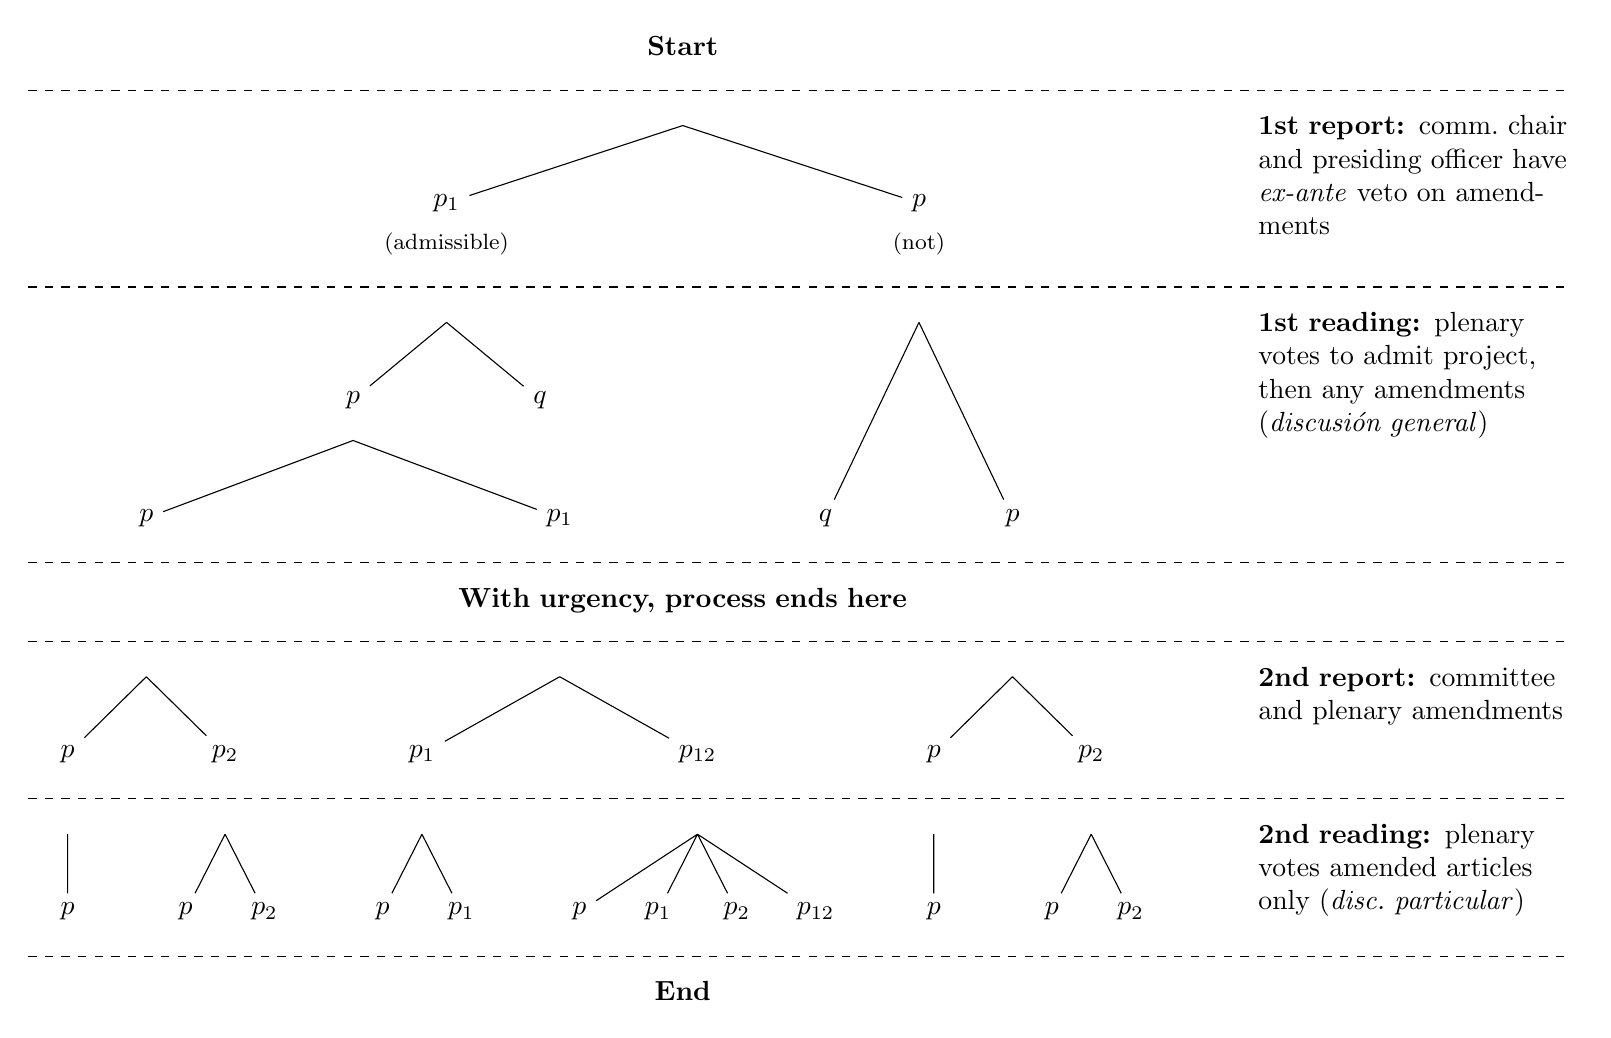
\begin{tikzpicture}
      \node[text width=10cm, text centered, anchor=north,fill=white] at (8.8125,-11) {\textbf{End}}; 
      %%%%%%%%%%%%%%%%%%%%%%%%%%%%%%%%%%%%%%%%%%%%%%%
      \draw[dashed] (0.5,-10.8) -- (20,-10.8);
      %%%%%%%%%%%%%%%%%%%%%%%%%%%%%%%%%%%%%%%%%%%%%%%
      \node[below] at (1,-10)    (o1)  {$p$}; 
      \node[below] at (2.5,-10)  (o2)  {$p$}; 
      \node[below] at (3.5,-10)  (o3)  {$p_2$}; 
      \node[below] at (5,-10)    (o4)  {$p$}; 
      \node[below] at (6,-10)    (o5)  {$p_1$}; 
      \node[below] at (7.5,-10)  (o6)  {$p$}; 
      \node[below] at (8.5,-10)  (o7)  {$p_1$}; 
      \node[below] at (9.5,-10)  (o8)  {$p_2$}; 
      \node[below] at (10.5,-10) (o9)  {$p_{12}$}; 
      \node[below] at (12,-10)   (o10) {$p$}; 
      \node[below] at (13.5,-10) (o11) {$p$}; 
      \node[below] at (14.5,-10) (o12) {$p_2$}; 
      \draw (1,-9.25) -- (o1)
            (3,-9.25) -- (o2)
            (3,-9.25) -- (o3)
            (5.5,-9.25) -- (o4)
            (5.5,-9.25) -- (o5)
            (9,-9.25) -- (o6)
            (9,-9.25) -- (o7)
            (9,-9.25) -- (o8)
            (9,-9.25) -- (o9)
            (12,-9.25) -- (o10)
            (14,-9.25) -- (o11)
            (14,-9.25) -- (o12);
      \draw[dashed] (0.5,-8.8) -- (20,-8.8);
      \node[text width=4cm, anchor=north west,fill=white] at (16,-9) {\textbf{2nd reading:} plenary votes amended articles only (\emph{disc.\ particular})}; 
      %%%%%%%%%%%%%%%%%%%%%%%%%%%%%%%%%%%%%%%%%%%%%%%
      \node[below] at (1,-8) (i21) {$p$}; 
      \node[below] at (3,-8) (i22) {$p_2$}; 
      \node[below] at (5.5,-8) (i23) {$p_1$}; 
      \node[below] at (9,-8) (i24) {$p_{12}$}; 
      \node[below] at (12,-8) (i25) {$p$}; 
      \node[below] at (14,-8) (i26) {$p_2$}; 
      \draw (2,-7.25) -- (i21)
            (2,-7.25) -- (i22)
            (7.25,-7.25) -- (i23)
            (7.25,-7.25) -- (i24)
            (13,-7.25) -- (i25)
            (13,-7.25) -- (i26);
      \draw[dashed] (0.5,-6.8) -- (20,-6.8);
      \node[text width=4cm, anchor=north west,fill=white] at (16,-7) {\textbf{2nd report:} committee and plenary amendments}; 
      % %%%%%%%%%%%%%%%%%%%%%%%%%%%%%%%%%%%%%%%%%%%%%%%
      \draw[dashed] (0.5,-5.8) -- (20,-5.8);
      \node[text width=10cm, text centered, anchor=north,fill=white] at (8.8125,-6) {\textbf{With urgency, process ends here}}; 
      %%%%%%%%%%%%%%%%%%%%%%%%%%%%%%%%%%%%%%%%%%%%%%%
      \node[below] at (2,-5) (g11) {$p$}; 
      \node[below] at (7.25,-5) (g12) {$p_1$}; 
      \node[below] at (4.625,-3.5) (g1) {$p$}; 
      \node[below] at (7,-3.5) (g2) {$q$}; 
      \node[below] at (13,-5) (g3) {$p$}; 
      \node[below] at (10.625,-5) (g4) {$q$}; 
      \draw (4.625,-4.25) -- (g11)
            (4.625,-4.25) -- (g12)
%            (13,-4.25) -- (13,-5.25)
            (5.8125,-2.75) -- (g1)
            (5.8125,-2.75) -- (g2)
            (11.8125,-2.75) -- (g3)
            (11.8125,-2.75) -- (g4);
      \draw[dashed] (0.5,-2.3) -- (20,-2.3);
      \node[text width=4cm, anchor=north west,fill=white] at (16,-2.5) {\textbf{1st reading:} plenary votes to admit project, then any amendments (\emph{discusión general})}; 
      %%%%%%%%%%%%%%%%%%%%%%%%%%%%%%%%%%%%%%%%%%%%%%%
      \node[below] at (5.8125,-1) (i11) {$p_1$}; 
      \node[text width=2cm, text centered] at (5.8125,-1.75) {\footnotesize{(admissible)}}; 
      \node[below] at (11.8125,-1) (i12) {$p$}; 
      \node[text width=2cm, text centered] at (11.8125,-1.75) {\footnotesize{(not)}}; 
      \draw (8.8125,-.25) -- (i11)
            (8.8125,-.25) -- (i12);
      \draw[dashed] (0.5,.2) -- (20,.2);
      \node[text width=4cm, anchor=north west,fill=white] at (16,0) {\textbf{1st report:} comm.\ chair and presiding officer have \emph{ex-ante} veto on amendments}; 
      %%%%%%%%%%%%%%%%%%%%%%%%%%%%%%%%%%%%%%%%%%%%%%%
      \node[text width=10cm, text centered, anchor=north,fill=white] at (8.8125,1) {\textbf{Start}}; 
      %%%%%%%%%%%%%%%%%%%%%%%%%%%%%%%%%%%%%%%%%%%%%%%
    \end{tikzpicture}  \\
\end{sidewaysfigure}



